% don't remove the folling lines, and edit the defintion of \main if needed
\documentclass[../report.tex]{subfiles}
\providecommand{\main}{..}
\IfEq{\jobname}{\currfilebase}{\AtEndDocument{\biblio}}{}
% until here

%file for shortcuts

\newcommand{\nch}{\ensuremath{N_{\mathrm {ch}}\xspace}}
\newcommand{\Ncoll}{\ensuremath{N_{\mathrm {coll}}}}
\newcommand{\Npart}{\ensuremath{N_{\mathrm {part}}}}
\newcommand{\dNdeta}{\mathrm{d}N_\mathrm{ch}/\mathrm{d}\eta}
\newcommand{\snn}         {\ensuremath{\sqrt{s_{\mathrm {NN}}}}}
\newcommand{\kT}          {\ensuremath{k_{\mathrm {T}}}}

\newcommand{\pp}          {pp}
\newcommand{\pPb}         {pPb}
\newcommand{\pA}          {pA}
\newcommand{\PbPb}        {PbPb}
\newcommand{\AuAu}        {AuAu}
\newcommand{\CuCu}        {CuCu}
\newcommand{\pAu}         {pAu}
\newcommand{\dAu}         {dAu}
\newcommand{\lsim}        {\,{\buildrel < \over {_\sim}}\,}
\newcommand{\gsim}        {\,{\buildrel > \over {_\sim}}\,}
\newcommand{\co}[1]       {\relax}
\newcommand{\nl}          {\newline}
\newcommand{\el}          {\\\hline\\[-0.4cm]}

\begin{document}

\section{Emergence of Hot and Dense QCD in Small Systems}

\subsection{Historic overview}
% Comments wrt initial LHC program
% Table (-> Constantin, Naghmeh)

\subsection{Open questions and their theoretical implications}

% Nature of collectivity / initial vs final state
% Are “collective effects” caused by final-state interactions in pp and pPb? → we should see jet quenching and medium-quark interactions
%   RAA, X+jet correlations
%   HF vn, Strangeness enhancement
% (Smooth?) transition from pp to pPb to PbPb
% Is there a turn on of at low Nch?
%   Subevents
%   Higher order cn (may be hopeless..)
% Make clear why pp and pPb are needed
% Integrate different modelling approaches (hydro, CGC, escape, …) 
% Shortcomings of current modelling in small systems (need to argue how run 3 and 4 can improve this)

\subsection{Key observables}

\subsubsection{Multiplicity distribution in pp}

\todo{NB. This section will most likely be too long, and has to be shortened for the yellow report}
For the performance estimates at high multiplicity in pp, a multiplicity-distribution extrapolation has been used which is based on existing ALICE ($|\eta| < 1.5$) and ATLAS ($|\eta|< 2.5$) data. Data from CMS is compatible with the used distribution and is therefore not explicitly included in the extrapolation. A parameterisation with a single\footnote{At LHC energies two NBDs are needed for a good fit to the full distribution, but one is sufficient for the tail of the distribution.} negative binomial distribution is used which also have been frequently used to characterize the multiplicity distribution~\cite{GrosseOetringhaus:2009kz,ALICE:2017pcy}.

The data used is shown in Fig.~\ref{fig:smallsystems_mult_data}. The fit with a single negative binomial distribution of the tail of the distribution (XX\% of the cross-section) is also shown. The three parameters of this fit are shown as a function of centre of mass energy in Fig.~FIGURE together with a power-law fit used to interpolate to 5.5 TeV and extrapolate to 14 TeV.

\begin{figure}[ht]
\centering
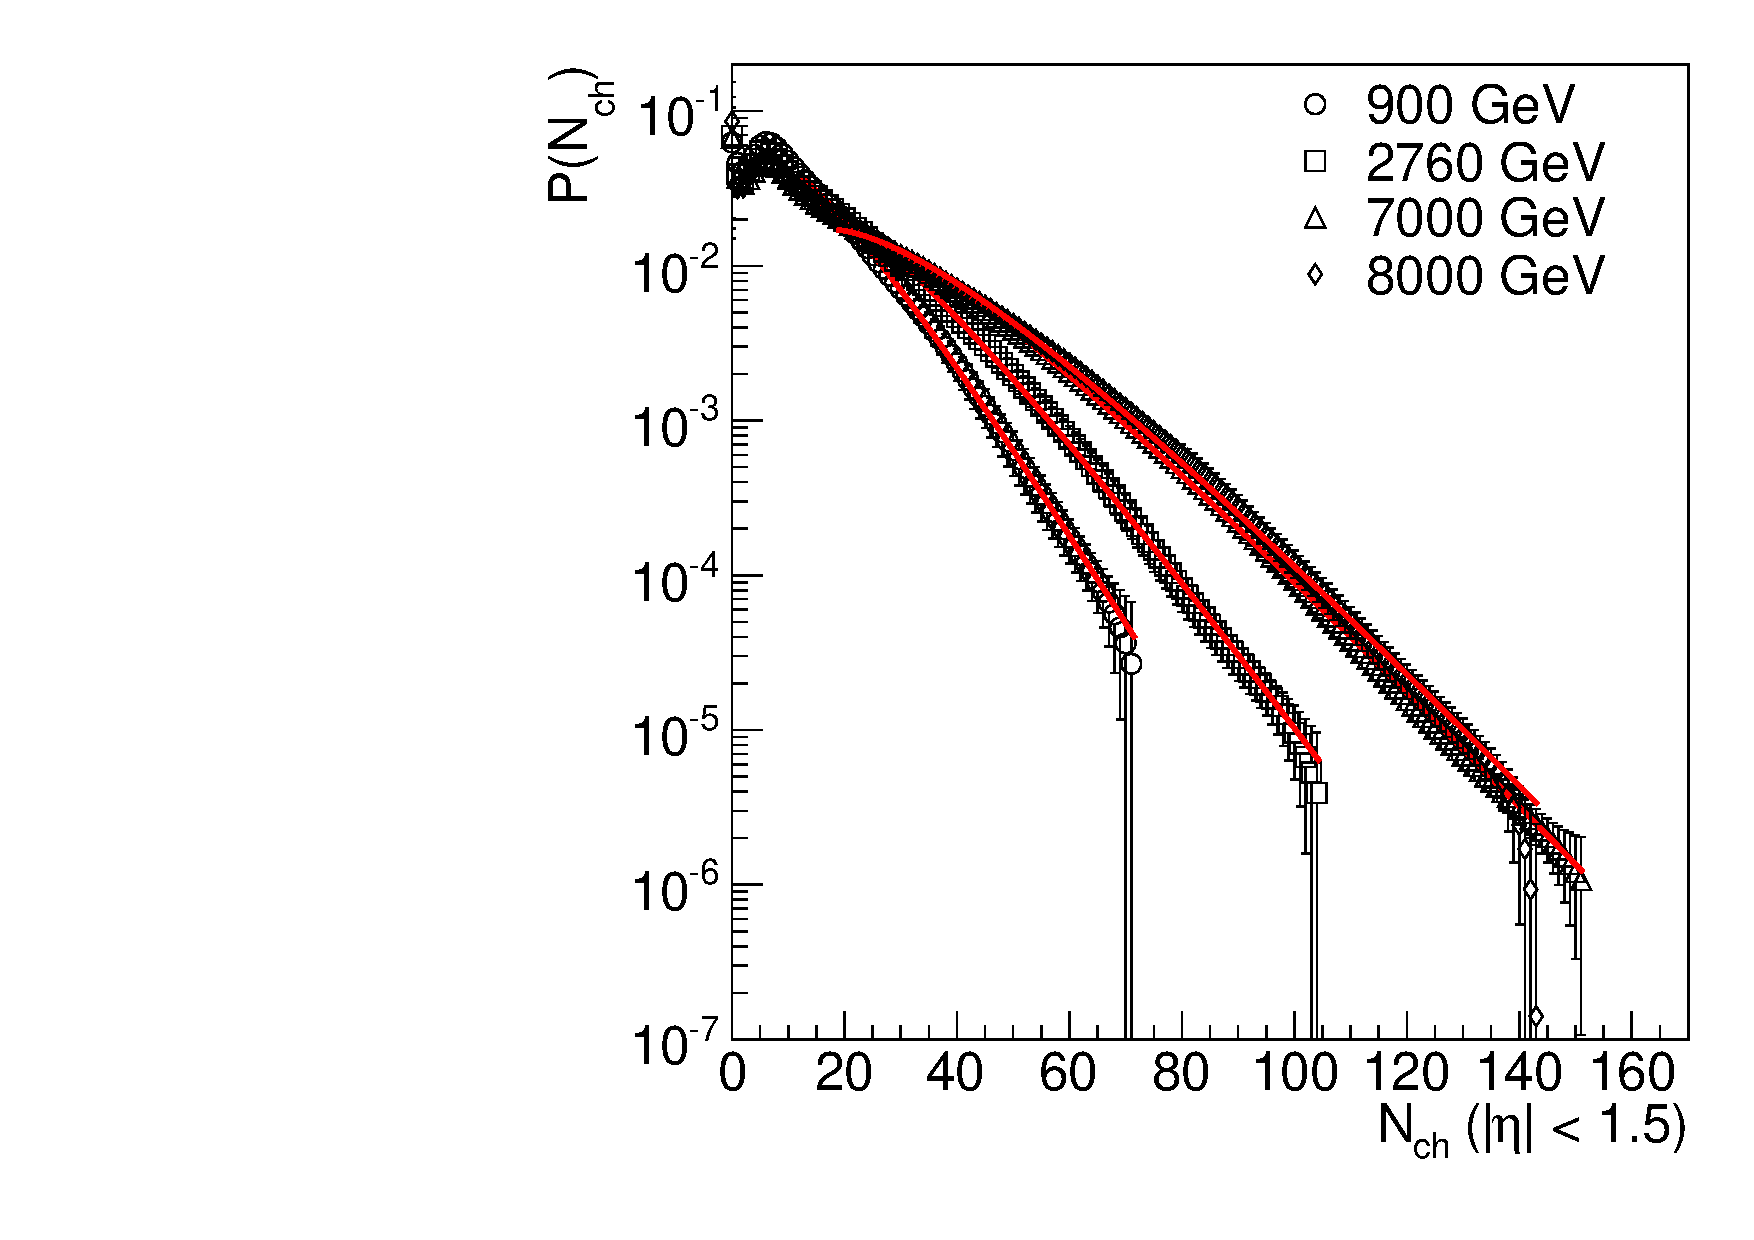
\includegraphics[width=0.49\linewidth]{\main/smallsystems/img/mult_data_1.pdf}
\hfill
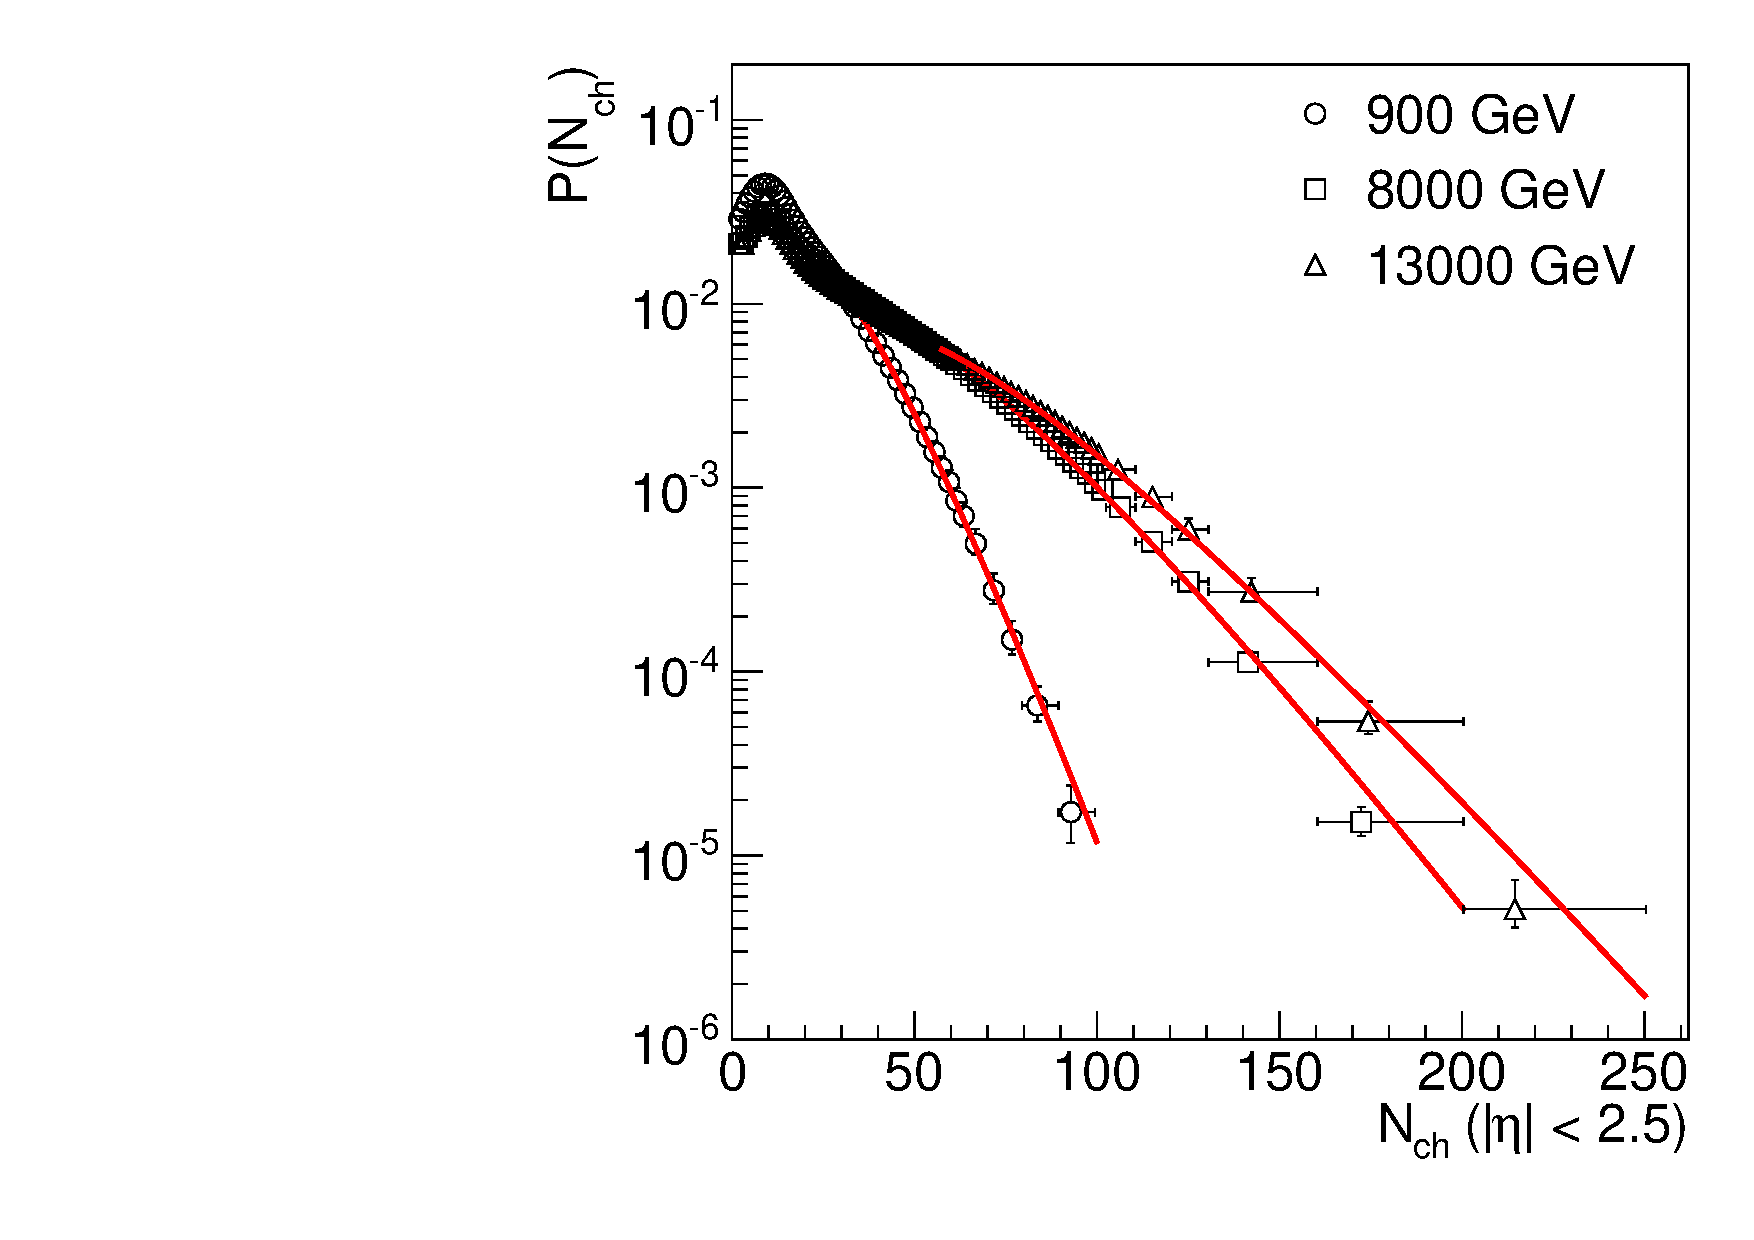
\includegraphics[width=0.49\linewidth]{\main/smallsystems/img/mult_data_11.pdf}
\caption{Multiplicity distributions measured by ALICE (left panel) and ATLAS (right panel) overlaid by the fit with a negative binomial distribution.}
\label{fig:smallsystems_mult_data}
\end{figure}

\begin{figure}[ht]
\centering
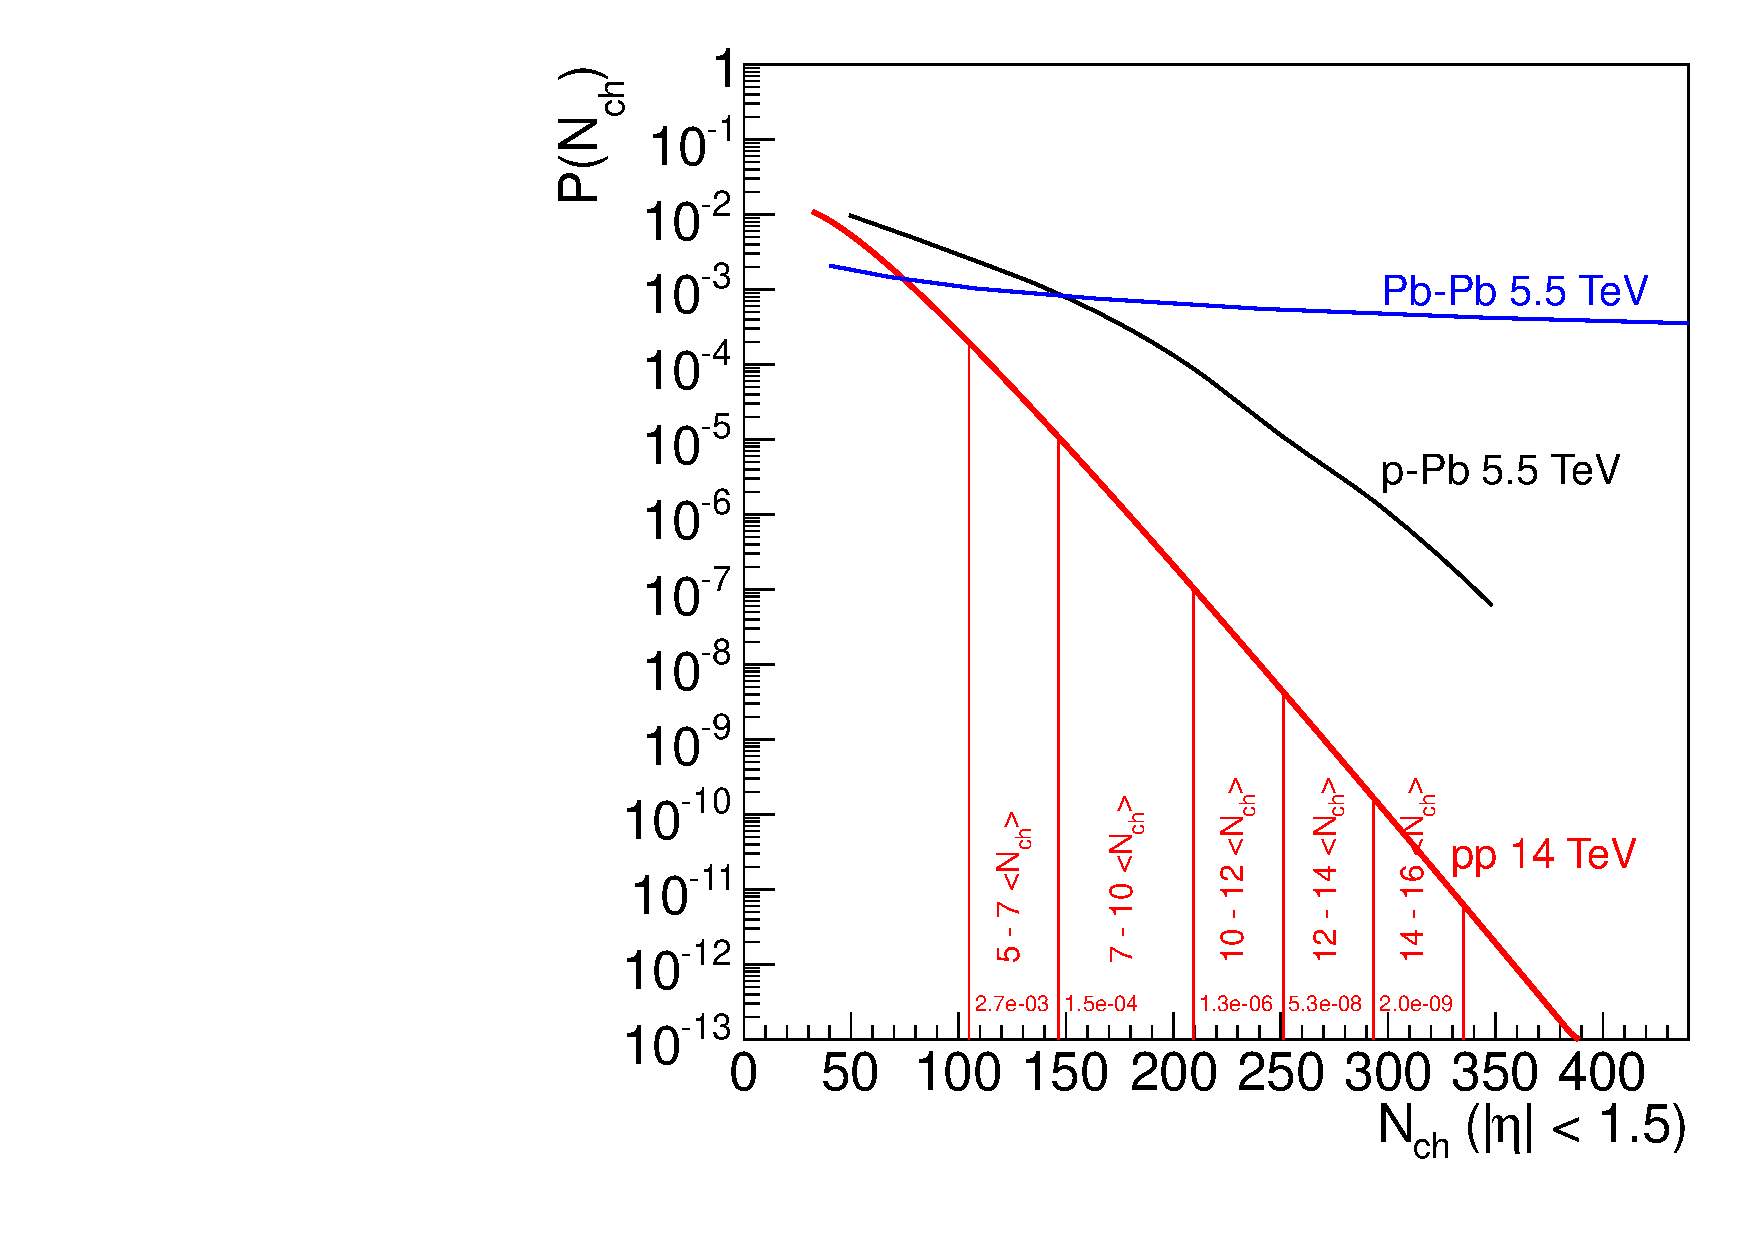
\includegraphics[width=0.32\linewidth]{\main/smallsystems/img/mult_extrapolation_1.pdf}
\includegraphics[width=0.32\linewidth,draft]{\main/smallsystems/img/mult_extrapolation_11.pdf}
\includegraphics[width=0.32\linewidth,draft]{\main/smallsystems/img/mult_extrapolation_11.pdf}
\caption{Extrapolated multiplicity distributions within $|\eta| < 1.5$ (left panel) and $|\eta| < 2.5$ (center panel) and scaled to the average multiplicity (right panel). The region of 14--16 \nch\ is indicated.}
\label{fig:smallsystems_mult_extrapolation}
\end{figure}

The resulting multiplicity distribution for 14~TeV is shown in Fig.~\ref{fig:smallsystems_mult_extrapolation} for the ALICE and ATLAS case. \todo{comment on comparison, and on general uncertainties of tail}. \todo{discuss comparison to pPb and PbPb}

\begin{table}
\centering
\begin{tabular}{c|c|c|c}
Range & $\dNdeta$ & Events per pb$^{-1}$ & Events in 200~pb$^{-1}$ \\
\hline
5--7 \nch     & 35--49   & 1.9e+08       & 3.7e+10 \\
7--10 \nch    & 49--70   & 1.0e+07       & 2.0e+09 \\
10--12 \nch   & 70--84   & 9.0e+04       & 1.8e+07 \\
12--14 \nch   & 84--98   & 3.7e+03       & 7.3e+05 \\
14--16 \nch   & 98--112  & 1.4e+02       & 2.8e+04 \\
\hline
\end{tabular}
\caption{Number of events in selected multiplicity bins.}
\end{table}

\begin{table}
\centering
\begin{tabular}{l|c|c|c}
Range & $\dNdeta$ & Events per pb$^{-1}$ & Events in 200~pb$^{-1}$ \\
\hline
0--5\% p--Pb   & 41--56        & 4.9e+07       & 9.8e+09 \\
5--10\% p--Pb  & 34--41        & 1.9e+08       & 3.8e+10 \\
10--20\% p--Pb & 27--34        & 6.6e+08       & 1.3e+11 \\
20--40\% p--Pb & 20--27        & 2.7e+09       & 5.4e+11 \\
\hline
60--65\% Pb--Pb    & 98--137       & 1.5e+02       & 3.0e+04 \\
65--70\% Pb--Pb    & 68--98        & 1.6e+05       & 3.1e+07 \\ 
70--75\% Pb--Pb    & 45--68        & 2.1e+07       & 4.2e+09 \\
75--80\% Pb--Pb    & 29--45        & 5.9e+08       & 1.2e+11 \\
80--85\% Pb--Pb    & 18--29        & 4.6e+09       & 9.1e+11 \\
\hline
\end{tabular}
\caption{Number of events in pp collisions sliced in equivalent multiplicity bins in p--Pb and Pb--Pb collisions.}
\end{table}


\todo{where to add which sigma(pp) used}

\subsubsection{Particle Correlations}

The measurements of two-particle correlations and higher-order cumulants have produced the initial observations of collectivity in small systems. In pp collisions, two distinct regions are of interest at HL-LHC: the high-multiplicity tail and the low-multiplicity regions. 

In pPb collisions, ...

\begin{figure}[ht]
\centering
\includegraphics[draft]{\main/smallsystems/img/corr_cumulants.pdf}
\caption{Higher-order cumulants with and without applying subevents for pp (left) and pPb (right) as a function of Nch. ATLAS.}
\label{fig:smallsystems_corr_cumulants}
\end{figure}

\begin{figure}[ht]
\centering
\includegraphics[draft]{\main/smallsystems/img/corr_symmetriccumulants.pdf}
\caption{Symmetric cumulants extracted with and without applying subevents for pp (left) and pPb (right) as a function of Nch. CMS.}
\label{fig:smallsystems_corr_symmetriccumulants}
\end{figure}

\begin{figure}[ht]
\centering
\includegraphics[draft]{\main/smallsystems/img/corr_cumulants_pid.pdf}
\caption{Particle identified $v_n$ (TODO only v2?) coefficients for pi, K, p (pp, ALICE), D mesons (pp, CMS), J/Psi (pp, pPb, ALICE, CMS) as a function of pT. Note that the multiplicity ranges are different for the different estimates. TODO: Plot may be messy and may need splitting in several panels.}
\label{fig:smallsystems_corr_cumulants_pid}
\end{figure}

\begin{figure}[ht]
\centering
\includegraphics[draft]{\main/smallsystems/img/corr_pvn.pdf}
\caption{P(vn) estimate (ATLAS/ALICE).}
\label{fig:smallsystems_corr_pvn}
\end{figure}

\subsubsection{Strangeness Enhancement}

\begin{figure}[ht]
\centering
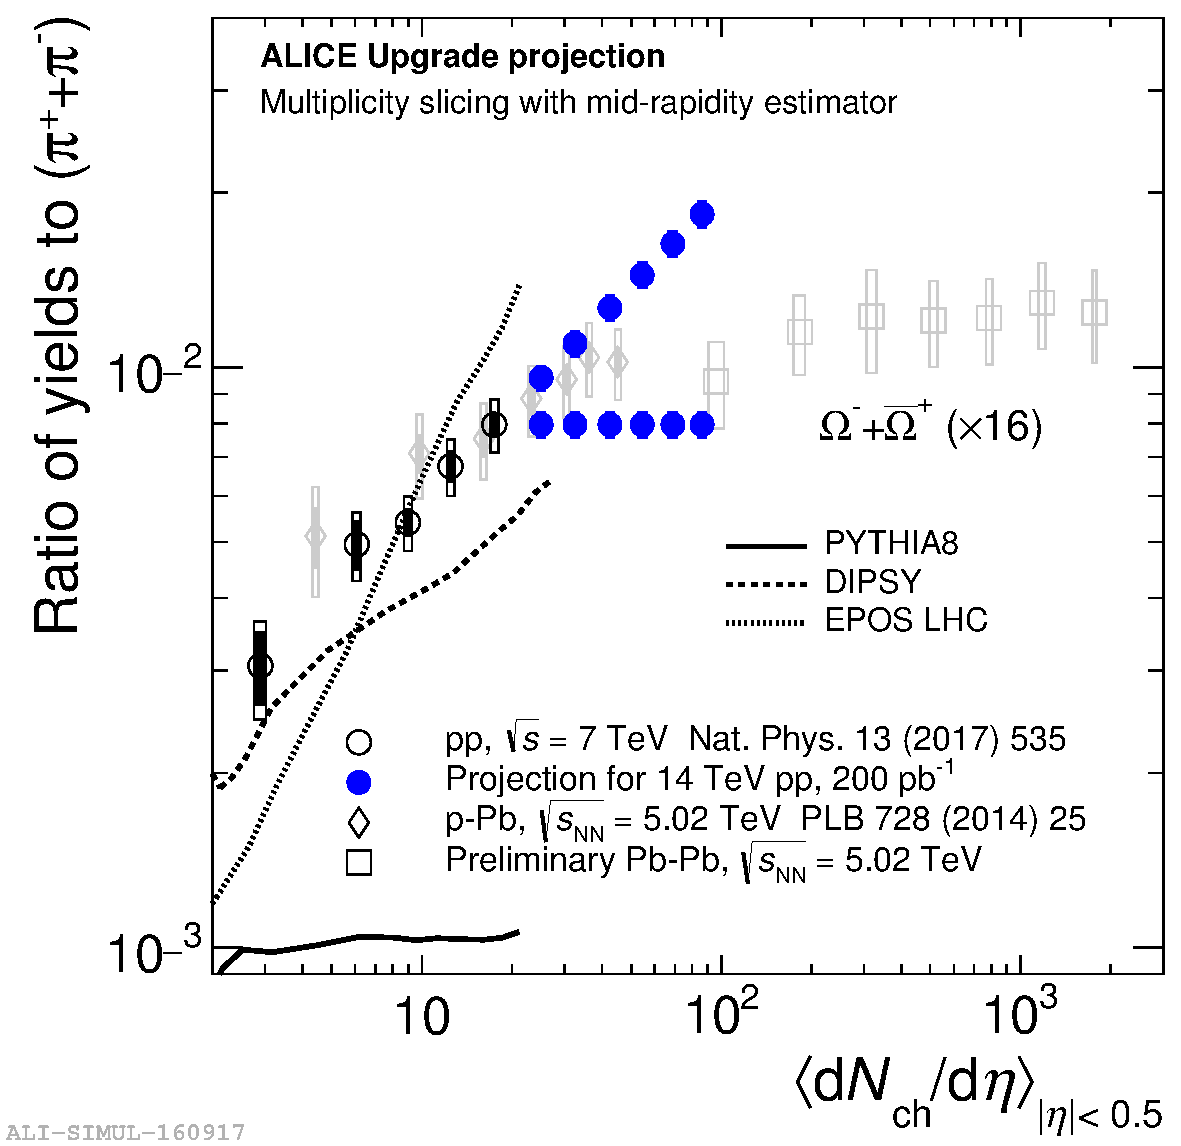
\includegraphics[height=9cm]{\main/smallsystems/img/strangeness_omegapi.pdf}
\caption{$\Omega/\pi$ ratio as a function of $\nch$ in pp collisions. Black symbols denote existing data \cite{ALICE:2017jyt} and blue symbols extrapolation. TODO add syst unc scaled by factor 2}
\label{fig:smallsystems_strangeness_omega_pi}
\end{figure}

\subsubsection{Energy Loss}

Narrative: 
- Existing pA eloss measurements (ALICE, ATLAS, CMS) show limit of maximal few percent quenching. In conclusion, RpA is not a good observable
- Produce estimates for a) h-jet (a la ALICE), b) gamma-jet or Z-jet (ATLAS/CMS), c) jet substructure
- Produce these for pA and pp
- For pp, see if high mu sample can be also used for something. In fact it should be made clear where it can be used and where not, as this chapter will be one of the places where a low mu pp program is motivated.

\begin{figure}[ht]
\centering
\includegraphics[draft]{\main/smallsystems/img/energyloss_hjet.pdf}
\caption{Modification of jet recoil yields extracted from hadron-jet correlations for pp collisions (left) and p-Pb collisions (right). Delta-recoil ratio vs. pT.}
\label{fig:smallsystems_energyloss_hjet}
\end{figure}

\begin{figure}[ht]
\centering
\includegraphics[draft]{\main/smallsystems/img/energyloss_Zjet.pdf}
\caption{Z-jet correlations in pp (left panel) and p-Pb collisions (right panel). 1/N dN/dxZj vs xZj.}
\label{fig:smallsystems_energyloss_Zjet}
\end{figure}

\subsubsection{Thermal Radiation}

\begin{figure}[ht]
\centering
\includegraphics[draft]{\main/smallsystems/img/thermal_radiation.pdf}
\caption{Thermal dileptons. dN/Mee vs. Mee}
\label{fig:smallsystems_thermal_radition}
\end{figure}

\subsection{Data-taking strategy}

% High multiplicity triggering, pile up, MB sample
% pp
%   ALICE: additional several month pp program
%   ATLAS/CMS: special runs (mu~1) or special conditions at end of fill
%   LHCb: either in nominal (mu~5) or special running
%   HM sample: 200 pb-1 pp (per experiment)
%   How much MB for low-multiplicity questions?
% p-Pb scheduled run
%   1000-2000 nb-1

\subsection{Summary}

\end{document}
